\documentclass[12pt]{article}

\usepackage{amssymb}
\usepackage{graphicx}
\usepackage{pgfplots}
\usepackage{rotating}
\usepackage{tikz}
\usepackage{xcolor}
\usepackage{setspace}

\usetikzlibrary{shapes.geometric, arrows}
\graphicspath{ {./images/} }
\pgfplotsset{width=10cm, compat=1.9}

\tikzstyle{block} = [
    rectangle, rounded corners, minimum width=5cm, minimum height=0.8cm,
    text centered, draw=black
]
\tikzstyle{hot-block} = [
    rectangle, rounded corners, minimum width=5cm, minimum height=0.8cm,
    text centered, draw=black, fill=red!30
]
\tikzstyle{arrow} = [thick,->,>=stealth]

\begin{document}

\begin{titlepage}
    \begin{center}
        \vspace*{1.5in}

        \Huge
        Using the GPU to Accelerate Non-Destructive Image Editing

        \vspace*{2in}

        \Large

        Trinity Term 2022

        \vspace*{0.25in}
        Candidate Number: \emph{1034710}

        \vspace*{0.25in}
        Masters in Computer Science
    \end{center}
\end{titlepage}



\pagebreak

\tableofcontents



\doublespacing

\pagebreak

\section{Introduction}

\subsection{Goal}

When image editing, the user's mental model of an edited image corresponds roughly to a sequence of
layers, where each layer can be passed through any number of `filters', which are operations which
modify these layers (e.g. by moving, rotating, sharpening, adding blur, tweaking colours, etc.).
The `filtered' versions of these layers are finally merged (or `composited') together to form the
final `composite' image that the user sees.

The ideal user experience for an image editor is one where, internally, the editor uses precisely
this model and exposes it to the user.  Additionally, when the user makes changes, the ideal image
editor would instantly updates the composite image on their screen.  `Instant' means that the update
latency is imperceptible, ideally within 16.6ms so that the new image can be rendered in the same
frame as the GUI is updated (consistently rendering in under 16.6ms allows the editor to run at 60
frames per second).

No existing image editor provides anything similar to this user experience.  However, designing and
implementing a production-ready image editor from scratch is well outside the scope of a university
project, so the goal is instead to \emph{prove the concept} by designing, implementing and
benchmarking a prototype image editing library.

\subsection{Challenges}

The obvious challenge of non-destructive image editing is the amount of computation work
required to update images.  Most images contain several million pixels, so updating the image
requires performing millions of individual computations whenever the user makes a change.  

Almost all modern computers have two different processors: a Central Processing Unit (CPU) which is
very fast and flexible and designed for sequential tasks, and a Graphics Processing Unit (GPU) which
is designed specifically to be extremely fast at 2D and 3D graphics and other highly parallel tasks.
Image editing is such a highly parallel task, which means that an image editor can be easily
\emph{GPU-accelerated}.  That is, every time there is an edit, the CPU sends a set of commands to
the GPU to perform the computation, and lets the GPU do all the image processing.  Contrasting this
with using the CPU exclusively, using GPU-acceleration means we can simultaneously use both
processors for what they are best at---the CPU is optimised for general-purpose computation on a
small amount of data (in this case, the image tree), whereas the GPU is optimised for highly
parallelisable tasks (in this case, the actual image processing).

The resulting speedup is very significant: on a desktop PC with a dedicated graphics card, graphics
processing is about \textbf{28x} faster on the GPU than the CPU.  On a laptop with integrated
graphics and limited power consumption, the difference is more like 3x.  GPU acceleration largely
solves the computation problem---each filter pass on a 2-million-pixel image takes roughly 0.2ms on
a dedicated GPU---but GPU-acceleration comes at the cost of significantly increased complexity.
Additionally, moving the computation to a largely opaque computing device makes debugging and
profiling significantly more difficult.

Therefore, the true challenge in this project comes in designing and implementing an GPU-accelerated
image editor in a way that is intuitive for the user and is simple enough for the code to be
possible to maintain.

\subsection{Contribution}

This project presents a novel approach to implementing image editors, where \emph{all} the image
processing is performed on the GPU.  Once an image tree has been `loaded' (i.e. all its textures and
assets sent to the GPU), updating the tree only requires the CPU to generate a sequence of GPU
commands which will then be executed asynchronously.  This design also presents an improved user
experience, where there are no boundaries to the sizes of layers---the user simply specifies what
filters to apply and the editor determines the correct sizes for the intermediate textures.

The approach for generating GPU commands is very similar to that of multi-pass compilers: we convert
the abstract image tree to GPU commands via in `intermediate' format, which provides extra
annotations such as which concrete textures to use.  Additionally, an algorithm is presented for
computing the bounding boxes of the regions of the intermediate textures that actually need to be
processed.  Skipping irrelevant computation results in significantly less computation required from
the GPU.

A prototype this approach has been designed and implemented in Rust, using WebGPU's graphics API.
The resulting prototype is fully portable and can run on any of the major OSes (Windows, macOS,
Linux, iOS and Android).  Whilst lacking many features expected of a production ready image editor
(such as a GUI), this shows that the core idea works and is possible to write in a way that is
maintainable.

Finally, this prototype has been used as a benchmark to compare the performance of image processing
on various computers (laptop or desktop) and compute devices (CPU, GPU compute or GPU rendering).
On the desktop, GPU rendering is \textbf{28x} faster than the CPU and performing a single filter on
a 2 million pixel image takes roughly 0.2ms.  Therefore, nearly 80 image operations can be applied
within the 16.6ms frame budget.  A laptop is, as expected, much slower (about 7x slower) but GPU
rendering can still perform a 2-million pixel image filter in about a millisecond.

If the results of previous computations are cached, then only the operations directly affected by a
modification need to be recomputed.  Therefore, on current-generation laptops, images with up to 10
stacked filters will still be able to hit 60 frames per second.  Desktop machines with discrete
graphics cards can comfortably perform roughly 80 stacked filters without dropping frames.

\subsection{Report Outline}

Section~\ref{sec:background} gives a detailed description of the background topics which are
relevant to this project, including a comparison of different ways of processing images (CPU, GPU
compute and GPU rendering) and a comparison of different APIs for controlling GPUs.

In Section~\ref{sec:existing-editors}, we look at existing image editing projects (Photoshop,
Darktable and the GNU Image Manipulation Program) and discuss how none satisfy the goals of this
project.  We also look to these for inspiration on how (or how not) to implement a fully
non-destructive image editor.

In Section~\ref{sec:implementation}, we present the implementation of a proof-of-concept prototype
for a non-destructive image editor.  We also discuss some of the expected features of a
production-ready image editor that are intentionally omitted from the prototype.

In Section~\ref{sec:measurements}, we present and discuss results measuring the speeds of various
compute methods, using the prototype's brightness/contrast implementation as a benchmark.

Finally, in Section~\ref{sec:conclusion}, we conclude the report and propose similar projects
related to non-destructive GPU-accelerated image editing that would benefit from future work.



\pagebreak

\section{Background}\label{sec:background}

\subsection{Terminology}

\subsubsection{Image Model}

This project uses a model of image editing where an `edited' image is represented as a sequence of
source layers (i.e. existing images) which are composited (see Figure~\ref{fig:compositing})
together to form a final `composite' image.  On each layer can be applied any number of `filters',
which modify their input layer in some predictable way (for example, moving it, adjusting its
colours, blurring it, etc.).

In this report, we don't often refer to any other type of images, so the composite image is often
referred to as simply `the image'.

\subsubsection{Filter Types versus Filter Instances}

Intuitively, a filter \emph{type} is a generic version of a filter which is waiting for parameters,
whereas a concrete filter \emph{instance} supplies those parameters.  Therefore, `Gaussian blur',
`brightness/contrast' and `colour invert' are all filter \emph{types} (and are generic over some
parameters), whereas `Gaussian blur of radius 10 pixels' is a specific \emph{instance} of the
`Gaussian blur' \emph{type}.

Mathematically, a filter \emph{type} is a pair $(f, P)$ where $f: P \times \verb|image| \rightarrow
\verb|image|$ and $P$ is the set of possible parameters for the filter.  Each filter \emph{instance}
corresponds to a filter type $(f, P)$ and specific parameters $p \in P$.  Therefore, the result of
applying a filter \emph{instance} $((f, P), p)$ to an image $i$ is $f(p, i)$.

\subsubsection{Intermediate Textures versus Intermediate Layers}

In this project, there is a distinction between layers and textures: a texture is a concrete and
finite piece of data stored in the GPU's memory, while a layer is a conceptually infinite image.

Often, a layer will contain an image in some region and have transparency off to infinity in every
direction.  The unbounded nature of layers makes them impossible to compute directly, so instead we
store a finite region of the \emph{layer} in a \emph{texture}.

\subsection{Image Processing}

Image editors will largely be performing one of three types of operation:

\begin{enumerate}
    \item Per-pixel filters, where each pixel in the output is a simple function of either the same
        pixel in the input (e.g.\ brightness/contrast, hue/ saturation/value) or the pixels near it
        (e.g.\ pick/hurl noise, edge detect/sharpen, small blurs).
    \item Transformations, where the image is translated, rotated or distorted in some way.
    \item Compositing, where a large number of `layers' are merged to form one final image.  See
        Figure~\ref{fig:compositing}.
\end{enumerate}

\begin{figure}
    \begin{center}
        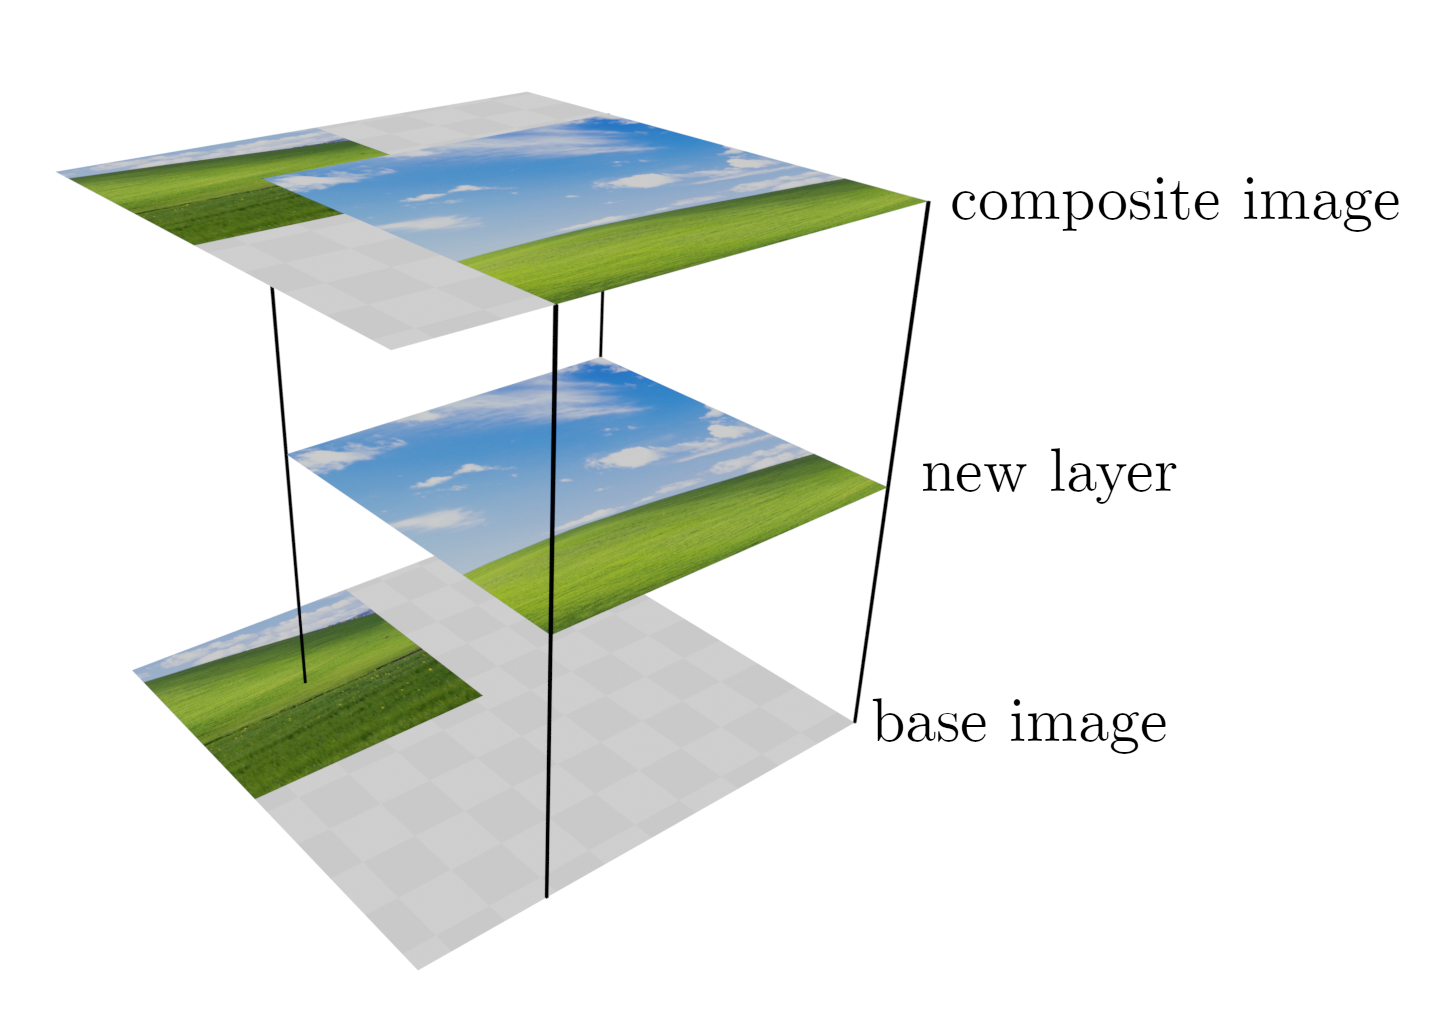
\includegraphics[width=0.6\textwidth]{compositing}
    \end{center}
    \caption{Compositing layers.  A base image is combined with a new layer (which only covers part
    of the image) to form a new image, with the new layer `above' the existing image.  Note how the
    top-left corner of the `new' image has overwritten the corner of the texture in base
    image.}\label{fig:compositing}
\end{figure}

All three of these are embarrassingly parallel---in each case, every pixel of the output can be
computed independently to all the others.

There are some image filters (like the various kinds of blur) which aren't as obviously
parallelisable, but there is still parallelisation opportunities (like computing 2D Gaussian blur by
combining horizontal and vertical blur passes, where each row/column is independent).



\subsection{Methods of Processing Images}\label{sec:compute-types}

In a typical consumer computer, there are two main processors which could be used for processing
images:

\subsubsection{The Central Processing Unit (CPU)}\label{sec:cpu}

Every computer contains a primary processor (the `Central Processing Unit' or CPU), which is
optimised for performing general computations on relatively small amounts of data.  There is some
parallelisation available, but CPUs are fundamentally optimised for fast sequential processing
rather than high parallelism.

Because of this, it's obvious that the CPU is a pretty inappropriate device for image processing.
The saving grace is that CPUs tend to have extremely high clock speeds and some degree of
parallelism: with multiple cores and SIMD, a modern CPU can be expected to perform upwards of 32
individual operations in parallel at roughly 3GHz\footnote{As of April 2022, CPUs have an average of
4.9 cores and almost all can perform 256-bit Single Instruction Multiple Data (SIMD) instructions.
So, 32 parallel operations can be achieved if 4 cores are each performing operations on eight 32-bit
floating-point SIMD lanes in a 256-bit AVX register.  However, limitations like memory speed and the
sharing of functional units (causing logically different threads to contest for the same hardware)
make this theoretical limit very difficult to reach in practice.  Data sourced from Steam's Hardware
Survey.}.  This is fast enough that CPU-based processing is \emph{passable} but the latency and
throughput are both far from ideal.  Additionally, maxing out a computer's CPU tends to have a
detrimental impact on other threads running on the same machine---including other parts of the image
editor, like the GUI thread.

\subsubsection{The Graphics Processing Unit (GPU)}\label{sec:gpu}

Almost all modern computers also contain a secondary processor, the Graphics Processing Unit (GPU),
who's sole purpose is to accelerate graphics processing with a low latency and high throughput.

Some form of GPU is present in nearly every consumer device, with even low-powered mobile devices
featuring GPUs integrated into the same piece of silicon as the CPU.  Therefore, we can confidently
rely on graphics acceleration being present when writing consumer applications.  Note that this has
only recently been the case---over the last two decades, rising screen resolutions and refresh
rates made dedicated graphics processing go from exclusive to gaming to being ubiquitous in consumer
devices.

An operation on a GPU can be performed in one of two ways, using either a \emph{render pass} or
a \emph{compute pass}:

\paragraph{Render passes:} Typically, a render pass involves taking 3D geometry, applying some
arbitrary transformation to the vertices, then performing some computation on every pixel of the
screen to compute its colour.  This is what GPUs are primarily designed for (it's what games need),
and is therefore GPUs have had many decades of optimisation relating to rendering efficiently.
Because rendering is a GPU's primary purpose, it means that render passes are available on any GPU.
Also, GPUs have fixed-function hardware to make rendering as fast as possible.

\paragraph{Compute passes:} Apart from the 3D rendering focussed render passes, modern GPUs also
allow execution of arbitrary code using \emph{compute passes}.  This is the basis for General
Purpose GPU (GPGPU) computing, and is largely driven by computationally demanding but highly
parallel tasks such as training neural networks.  Within the context of image editing, compute
passes are useful for doing operations that can't easily be represented as per-pixel operations,
usually the more complex filters such as Gaussian blur.

However, the generality of compute passes come at a cost: compute passes can't as easily make use of
the GPU's dedicated hardware for operations like sampling textures.  General-purpose compute is not
the primary purpose of a consumer GPU, so the lower-end or older a GPU gets, the less likely it is
for compute to work well.

In summary, \emph{compute} passes are much more general, but \emph{render} passes are much more
portable and often faster.  In general, if an operation can be written as a render pass then there's
rarely any point leaving it as a compute pass.  The prototype in this project uses entirely render
passes.

\subsection{Comparison of Compute APIs}

\subsubsection{CPU Compute (No API Needed)}

Computing images on the CPU is extremely simple, requiring no extra effort or clever APIs.  Source
images are loaded from disk into the CPU's memory as a flat array of pixel values.  Operations can
then be performed on those pixels using a plain \verb|for| loop.  Parallelisation can be achieved
using a combination of SIMD and multi-threading (splitting the pixels into chunks and having
different CPU cores process those chunks in parallel).  As described above in Section~\ref{sec:cpu},
CPUs are easy to program for but, on the whole, are ill-suited to the heavily parallel operations
found in image processing.

\subsubsection{Graphics Libraries}

Controlling GPUs directly is a hideously complex task, since you would be forced to deal with the
differences between every model of GPU.  To combat this, operating systems vendors (like Apple and
Microsoft) or the Khronos Group \cite{khronos} design APIs which provide users with a simpler
abstraction for the GPU, and require that GPU vendors implement this standard API in each GPU's
drivers.

The oldest and most well-known graphics API is OpenGL \cite{opengl}, first
released in in 1992 by the Khronos Group.  OpenGL is very high-level, which makes it easy to use for
simple cases (like making games) but lacks the low-level control required for achieving high
performance in more obscure cases (like image editors).

Armed with 24 years of hindsight, Khronos released Vulkan \cite{vulkan} in 2016 as a successor to
OpenGL.  Meanwhile, Apple and Microsoft released Metal \cite{metal} and DirectX \cite{directx},
respectively.  All of these modern APIs favour a lower-level approach, requiring more code from
their users but allowing much more fine-grained control and potential for much better performance.  

Until 2018, OpenGL and Vulkan where fully supported by all major operating systems (Windows, macOS,
Linux, iOS and Android).  However, in 2018, Apple announced that they would be deprecating OpenGL
(along with Vulkan and OpenCL) to encourage developers to use their own API, Metal.  As of 2022,
OpenGL, Vulkan and OpenCL all still work on Apple devices, but it is unclear for how long this will
continue.  Code using Vulkan can be used on Apple devices by using MoltenVK \cite{moltenvk} to
translate Vulkan function calls into Metal at runtime.  Similarly, MoltenGL \cite{moltengl} provides
support for OpenGL, but both of these only implement a subset of their corresponding APIs and are
less than ideal.  The compatibility of various APIs, along with OpenCL (discussed in
Section~\ref{sec:open-cl}) and WebGPU (discussed in Section~\ref{sec:wgpu}), is summarised in
Figure~\ref{fig:apis-vs-oses}.

\begin{figure}
    \begin{center}
        \begin{tabular}{ c | c c c c c }
                    & Windows & macOS & Linux & iOS & Android \\
            \hline
            OpenCL  & \checkmark & deprecated   & \checkmark & deprecated   & \checkmark \\
            OpenGL  & \checkmark & subset       & \checkmark & subset       & \checkmark \\
            Vulkan  & \checkmark & subset       & \checkmark & subset       & \checkmark \\
            Metal   &            & \checkmark   &            & \checkmark \\
            DirectX & \checkmark \\
            \hline
            WebGPU & \checkmark & \checkmark & \checkmark & \checkmark & \checkmark
        \end{tabular}
    \end{center}
    \caption{Compatibility table of APIs against major operating systems.  iOS and Android are less
       relevant to image editors, but are included for completeness.}\label{fig:apis-vs-oses}
\end{figure}

\subsubsection{OpenCL}\label{sec:open-cl}

OpenCL \cite{opencl} (not to be confused with Open\textbf{G}L) is a
framework for running general compute operations on any hardware, also designed by the Khronos
Group.  OpenCL lets you write parallelisable C or C++ code once, then delegate that code to any
compute device (be that a CPU, GPU or anything else) at runtime.  Thus, the compute code only needs
to be written once.

As with OpenGL and Vulkan, OpenCL was fully portable until 2018, when Apple has also deprecated
OpenCL along with OpenGL and Vulkan.  Unlike the graphics APIs, no one has yet made a compatibility
layer like MoltenVK or MoltenGL (as far as I'm aware), so Apple devices still need to be handled as
a special case.  Finally, OpenCL, by its very nature as a \emph{compute} API, is required to use
\emph{compute} passes for its processing which, as described in Section~\ref{sec:gpu}, are less
portable and often significantly slower than render passes.

\subsubsection{WebGPU}\label{sec:wgpu}

WebGPU \cite{webgpu} is an in-progress standard to provide web applications with low-level but safe
access to general-purpose GPU acceleration.  WebGPU feels very similar to Vulkan, and delegates to
Vulkan, Metal or DirectX.  Therefore, WebGPU is extremely portable, at the cost of not implementing
more obscure parts of those native APIs.  A Rust library, \verb|wgpu| \cite{wgpu}, implements the
WebGPU specification in a way callable from native language like C, C++ and Rust.  \verb|wgpu| forms
the core of Firefox's WebGPU implementation, and is therefore very well-tested and stable.



\pagebreak

\section{State of the Art}\label{sec:existing-editors}

\subsection{Adobe Photoshop}

I don't think Photoshop needs much of an introduction, since it has a near monopoly over image
editing---to the point where its name is synonymous with image editing itself.  To give an idea of
just how dominant Photoshop is, it has an estimated 26 million users
world-wide \cite{photoshop-users}, including
90\% of the world's creative
professionals \cite{adobe-facts}.

\subsubsection{Non-Destructive Editing}

Since the introduction of Smart Objects \cite{smart-obj} (and the corresponding Smart Filters) in
2014, Photoshop has been able to implement most filters non-destructively.  These are all computed
on the CPU, though, so extensive use of Smart Filters will often cause Photoshop to become
noticeably slow and cause a noticeable bloat to the file size.

\subsubsection{GPU Acceleration}

Photoshop runs almost all of its image processing on the CPU.  As of 2022, nine operations benefit
from GPU acceleration, whilst a further eight \emph{require} a GPU \cite{photoshop-gpu}.  It makes
sense that the Photoshop is not built with GPUs in mind---the first version of Photoshop was
released in 1990 \cite{photoshop-wiki}, nine years before the first consumer GPU (Nvidia's GeForce
256) reached the market in 1999 \cite{first-gpu}.

Without access to Photoshop's source code, it's unclear exactly what APIs are being used this
GPU-acceleration.  Photoshop has settings for OpenCL, OpenGL, Vulkan and Metal, so I can only assume
that a combination of all four are used.  In summary, Photoshop appears to use largely CPU, with a
small amount of GPU compute passes and GPU rendering passes.

\subsection{GNU Image Manipulation Program (GIMP)}

The GNU Image Manipulation Program \cite{gimp} (shortened to GIMP) is a free and open
source general-purpose image editor.  It has largely dominated the space of free image editors, and
image editing on Linux (both areas where Photoshop chooses not to compete).

\subsubsection{Non-Destructive Editing}

As of 2022, all filters in GIMP are destructive, so there is no way to do non-destructive editing.
There is a plan to implement non-destructive editing \cite{gimp-faq} but that has not yet come to
fruition.  It appears that GIMP's code is not written with non-destructive editing in mind, so the
change appears to involve a monumental refactoring task.

\subsubsection{GPU Acceleration}

GIMP has experimental support for GPU acceleration via OpenCL (first released in 2.10.0
\cite{gimp-2.10} in April 2018).  As of 2022, this is still experimental and is sometimes slower
than CPU-based processing.  So, for most users, GIMP is 100\% CPU-bound.

\subsection{Darktable}

Darktable \cite{darktable} is an open source `photography workflow application'
which features non-destructive editing which can be performed entirely on the GPU.  The only thing
really missing is that Darktable only supports a fixed pipeline of filters, rather than allowing the
user to choose how to compose them (this makes sense, because Darktable is only intended to be used
for adjusting photos).  Finally, Darktable uses OpenCL which, as described above in
Section~\ref{sec:open-cl}, is deprecated on Apple devices and can't take advantage of the
portability and speed improvements of using render passes.



\pagebreak

\section{Implementation}\label{sec:implementation}

\subsection{Technologies Used}

The editing library is written in Rust, using \verb|wgpu| (see Section~\ref{sec:wgpu}) as the
graphics API\@.  \verb|wgpu| is an excellent library for this purpose---it provides low-level
control of the GPU in a way that is safe and runs on any major platform.  Not using native APIs
directly does create some overhead, but for a proof of concept the difference is negligible and the
portability and ease of use easily outweigh any small performance hit.  At any rate, there are many
better ways to optimise the prototype than using a different graphics library.

I also used WGSL (WebGPU's shading language) to write the shaders for the filters.  GLSL would
potentially have been easier, but the prototype doesn't need any complex shader logic and
\verb|wgpu|'s tutorials use WGSL so that's what I learned.

Finally, this report is written in \LaTeX\ and the 3D diagrams were made using a combination of
Blender \cite{blender} and GIMP \cite{gimp}.

\subsection{Notable Omissions}\label{sec:omissions}

This project is concerned with \emph{proving a concept} rather than with building a production-ready
image editor.  So, as such, many features that would be expected of a real image editor have been
omitted, since they would not change the feasibility of a fully GPU-accelerated image editor.  This
section highlights the largest of those omitted features.

\subsubsection{Gaussian Blur and Other Blurs}

Running Gaussian blur efficiently on GPUs has been very thoroughly researched \cite{fast-blur}
because of the applications in video games (for filters like bloom and depth of field) and GUIs and
the best algorithms, while slower than simple per-pixel filters, are very fast.  Approximation
techniques such as Kawase blur and Dual blur \cite{kawase-blur} give accurate results very quickly
(though they are still approximations).  Other blur-like operations (bloom, motion blur, glare,
etc.) are also prevalent in video games and variants of Kawase blur can also be used to compute
these efficiently.  

\subsubsection{Brushes and Undo/Redo}

Brush systems and handling undo/redo are simply out of scope.  Implementing either in a GPU-friendly
way are, in their own right, worthy of projects but \emph{this} project is primarily concerned with
measuring the speed of processing image filters (processing brushes and undo/redo happen
occasionally, whereas image filters need to be processed many times per frame).  Handling brushes
and undo/redo are unlikely to have much impact on this because they both involve occasionally
modifying the source image textures.

Similarly, implementing a GUI is also out of scope.

\subsubsection{Caching}

Strategically caching the intermediate results of computations is a very effective way of reducing
the time required to update an image.  It is also particularly effective in practice, since when the
user makes lots of consecutive edits, they are almost always applied \emph{in the same place} of the
tree.  Thus, caching the intermediate layer just below this point will provide a large performance
boost.

For example, think about the user dragging a slider in a filter.  This will cause the image to
update nearly every frame, but all these updates will always change the same filter.  Therefore,
each frame the editor only has to recompute the filters on the path from the change to the root,
which will always be faster than recomputing the entire image from scratch.

The major downside of caching is the memory usage it requires.  However, a quick sanity check tells
us that this is unlikely to be a problem: firstly, the image editor is \emph{already} storing a lot
of textures in the GPU's memory (one for every source image, one for the final image and at least
two intermediate textures) so the relative impact of a few extra cache textures is less significant
than it first appears.  Secondly, and most importantly, GPUs are designed to handle lots of
textures.  Each pixel takes four bytes, and images are likely to be around 2,000~$\times$~1,000
pixels.  Naively storing such a texture would take at most 4~$\times$~2,000~$\times$~1,000 bytes =
8MB.  Even humble integrated GPUs usually have at least 1GB of RAM, which is enough to store several
hundred such textures.  Even this is an underestimate, because GPUs store compressed versions of the
textures and use dedicated hardware to decompress them on demand.

Whilst extremely effective, introducing caching makes the whole system substantially more complex.
It also doesn't make the performance any easier to evaluate---we are principally interested in
\emph{how much} image processing we can do within a frame, and adding a caching system will only add
noise to these measurement.

\subsection{Design}

\subsubsection{Lifetime of the Image Editor}

Before processing any images, the code must gain access to a GPU and initialise all the filter
types.  This involves mostly compiling the shader modules, but if filter types need any specific GPU
resources (like look-up textures) then those are also allocated here.

To initially load an image, all the referenced textures are read from disk, decompressed and copied
into GPU memory.  Once the textures are on the GPU, they can be freed from CPU memory.

Now, all the required resources are already on the GPU, so any updates to the image tree only
requires us to send the GPU a sequence of commands to recompute the new image.  The resulting
composite image ends up stored in a texture in GPU memory, ready to be rendered to the screen.
Determining a suitable sequence of GPU commands is where almost all of the complexity lies, and is
explained in detail in Section~\ref{sec:gpu-cmds}.  However, an efficient sequence of GPU commands
can be generated very quickly.

If the image needs to saved to a file, then the composite image texture can be copied back into CPU
memory, encoded and finally written to disk as a file.  Otherwise, the final composite image is left
as a texture in GPU memory, ready to be rendered to the user's screen in the next frame.

This control flow is summarised in Figure~\ref{fig:control-flow}.  Note now all the expensive
operations, like compiling shaders and copying data between CPU/GPU memory, have been pushed out of
the `hot' code (updating the image, which could need to be run every frame) and into the `cold' code
(loading/saving images, which will happen quite rarely).

\begin{figure}
    \begin{center}
        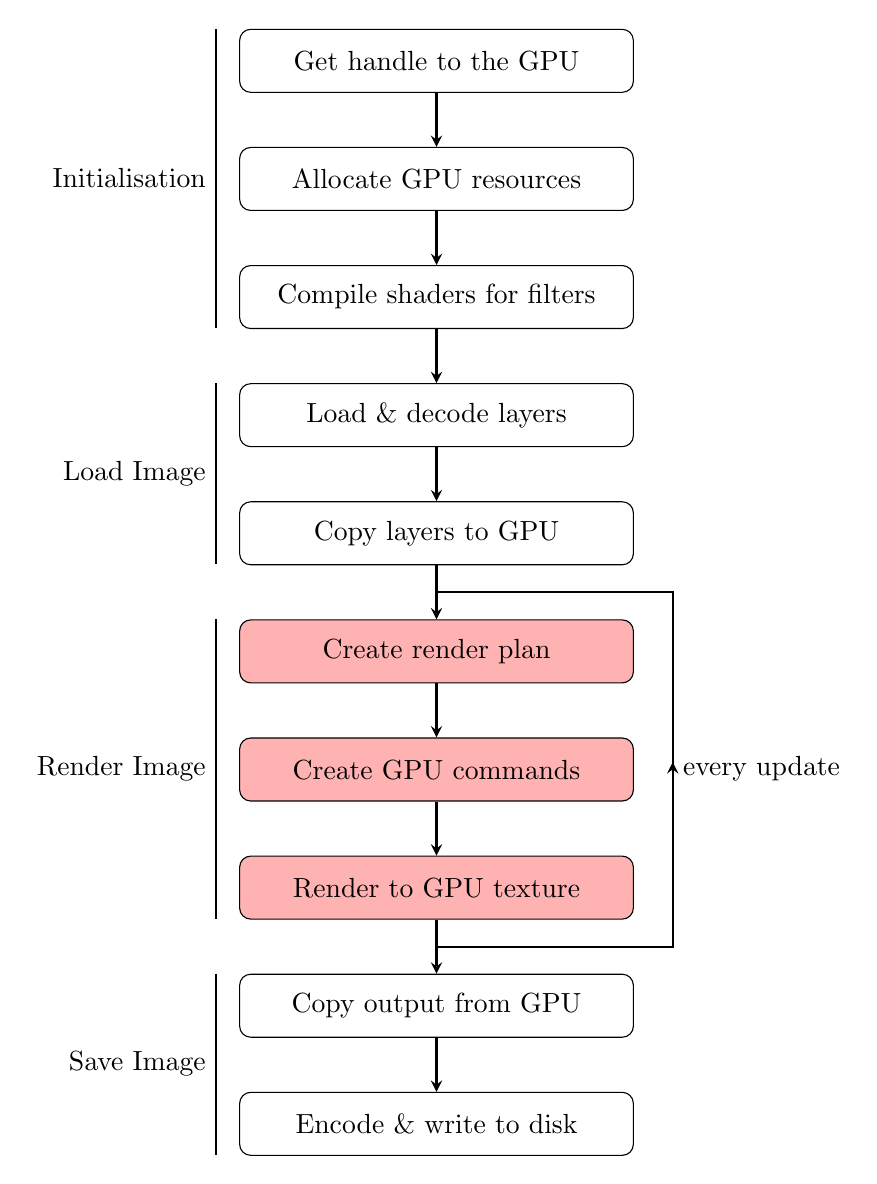
\begin{tikzpicture}[node distance=1.5cm]
            \node (init1) [block] {Get handle to the GPU};
            \node (init2) [block, below of=init1] {Allocate GPU resources};
            \node (init3) [block, below of=init2] {Compile shaders for filters};
            \draw [thick] (init1.north)+(-2.8,0) -- ++(-2.8,-3.8)
                            node[midway, anchor=east] {Initialisation};

            \node (load1) [block, below of=init3] {Load \& decode layers};
            \node (load2) [block, below of=load1] {Copy layers to GPU};
            \draw [thick] (load1.north)+(-2.8,0) -- ++(-2.8,-2.3)
                            node[midway, anchor=east] {Load Image};

            \node (render1) [hot-block, below of=load2  ] {Create render plan};
            \node (render2) [hot-block, below of=render1] {Create GPU commands};
            \node (render3) [hot-block, below of=render2] {Render to GPU texture};
            \draw [thick] (render1.north)+(-2.8,0) -- ++(-2.8,-3.8)
                            node[midway, anchor=east] {Render Image};

            \node (save1) [block, below of=render3] {Copy output from GPU};
            \node (save2) [block, below of=save1] {Encode \& write to disk};
            \draw [thick] (save1.north)+(-2.8,0) -- ++(-2.8,-2.3)
                            node[midway, anchor=east] {Save Image};

            \draw [arrow] (init1) -- (init2);
            \draw [arrow] (init2) -- (init3);
            \draw [arrow] (init3) -- (load1);
            \draw [arrow] (load1) -- (load2);
            \draw [arrow] (load2) -- (render1);
            \draw [arrow] (render1) -- (render2);
            \draw [arrow] (render2) -- (render3);
            \draw [arrow] (render3) -- (save1);
            \draw [arrow] (save1) -- (save2);

            \draw [arrow] (render3.south)+(0,-0.35) -- +(3,-0.35) -- +(3,2);
            \draw [thick] (render1.north)+(0,0.35) -- +(3,0.35) -- +(3,-1.9)
                            node[anchor=west] {every update};
        \end{tikzpicture}
    \end{center}
    \caption{Control flow of the image editor.  Note how only the {\color{red} red} blocks are
    contained with a loop; they are run every time the user makes a change to the image.  Thus,
    nearly all the editor's time will be spent in this loop, and it is always advantageous to move
    work out of the loop.}\label{fig:control-flow}
\end{figure}

\subsubsection{Generating GPU commands}\label{sec:gpu-cmds}

To `compile' an image tree into a sequence of concrete GPU commands, this project takes heavily
inspiration from multi-pass compilers: we start with an `abstract' tree representing the image, then
`lower' this tree into a new tree with more annotations, then finally `lower' this intermediate tree
again into precise GPU commands\footnote{For those familiar with compilers, these correspond
(respectively) to the Abstract Syntax Tree (AST), an Intermediate Representation (IR) and the final
machine code.}.  Comparing the intermediate tree to its abstract counterpart, the abstract tree is
designed to be a nice interface for the user of the library, whereas the intermediate tree is both
easier to optimise and easier to translate into GPU commands.

In the case of this prototype, the `lowering' of the Abstract Tree to the Intermediate Tree is
simply a matter of labelling each filter and layer source with what GPU texture it should use, as
well as a bounding box of the region that we actually need (see Section~\ref{sec:virt-tex-spaces}
for more about these regions).

Finally, once we know what regions of which textures to use, generating the GPU commands becomes
fairly simple: every filter type exposes a function with signature like

\begin{verbatim}
trait FilterType {
    ...

    fn add_commands(
        &self,
        in: TextureRegion, out: TextureRegion,
        command_encoder: &mut wgpu::CommandEncoder,
    );
}
\end{verbatim}

This declares a \verb|trait| containing a function with four arguments: \verb|&self| is equivalent
to the \verb|self| parameter in Python or \verb|this| in object-oriented languages.  \verb|&self|
means that \verb|self| is \emph{immutable} (as opposed to \verb|&mut self| which would be mutable).
\verb|in| and \verb|out| are two \verb|TextureRegion|s specifying the regions of virtual and actual
texture space on either side of the effect.  Finally, \verb|command_encoder| is a \emph{mutable}
reference to a \verb|wgpu::CommandEncoder|, to which the render/compute passes should be added.

For per-pixel effects, this simply requires rendering a single quad that covers the correct region
of the output layer.  Getting the various coordinates (the quad's vertices and texture coordinates)
right is fiddly but not difficult.

More complex filters, such as transformations or blurs, require special treatment, but this design
means they can each be implemented in isolation.  Additionally, the \verb|TextureRegion|s provide
the filters with all the information required to correctly sample the incoming textures.

\subsubsection{Virtual Texture Spaces}\label{sec:virt-tex-spaces}

When editing images, it is relatively common to encounter a situation where a layer is partially
outside the boundary of the whole image.  This presents an optimisation opportunity: sometimes we
only need to process filters for part of a layer, and if we can limit the size of the intermediate
textures, the processing will be faster because the GPU simply has to do less work.  In fact, there
are other ways that we can restrict the size of intermediate textures---any filter which throws away
information (masks, cropping, filling the layer with a solid colour, etc.) can also provide stricter
bounds for the filters below them.

Additionally, it would improve the consistency of the user experience if we are able to implement
transformation (translation, rotation, scaling, etc.) as \emph{just another filter}.  This allows
the user to intuitively create effects like stretching layers after blurring, as well as removing
layer positioning as a special case for the code to deal with.

It turns out that there's a simple way to achieve both of these: remove the requirement for the
origin of the intermediate textures to correspond to the origin of the larger layer they're trying
to represent.  I've dubbed these larger texture spaces `virtual', because the layer coordinates used
by the filters aren't anchored to any \emph{physical} texture.

This is illustrated in Figure~\ref{fig:virt-tex-space}.  See how the \verb|intermediate| textures
take up a rectangle in the middle of a larger texture space (in this case, the texture space of the
output image).  Also, see how the colour invert is only applied to the top-left region of
\verb|source_texture|, thus saving the GPU work.

\begin{figure}
    \begin{center}
        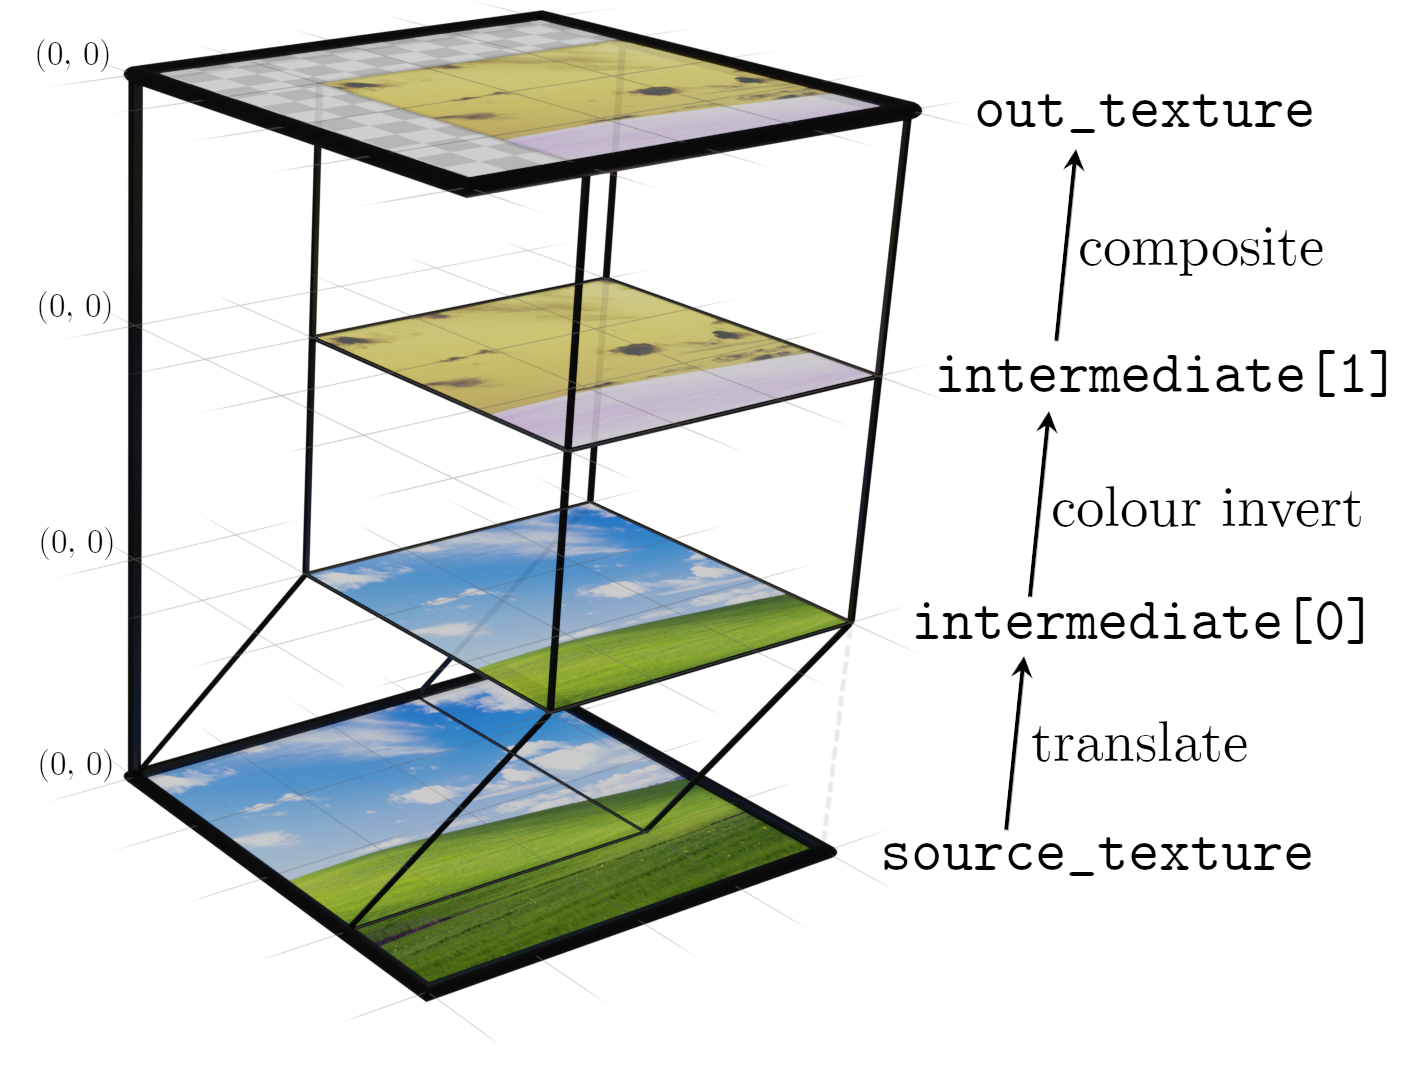
\includegraphics[width=0.9\textwidth]{filter-stacking}
    \end{center}
    \caption{Processing image filters using `virtual' texture space.  Note how the $(0, 0)$ points
    for both \texttt{intermediate} layers fall \emph{outside} the region stored in the
    texture.  Also note how the virtual texture spaces has allowed us to avoid processing nearly
    half of the source layer.}\label{fig:virt-tex-space}
\end{figure}

From the user's perspective, these virtual texture spaces are effectively infinite in every
direction.  By extension, this means that the user doesn't ever have to worry about layer
boundaries---the editor will automagically allocate enough texture space to fit the intermediate
layers.  If the user does somehow manage to create an enormous intermediate texture (e.g. by
scaling up by 1,000,000x, followed by scaling down by 1,000,000x), we can avert disaster by imposing
a maximum intermediate texture size and only storing a very low-resolution version of the oversized
layer.  It's unlikely that the user would notice the difference, because the output image almost
certainly contains less information than this intermediate texture---meaning that much of the extra
information has to be compressed out.  Possible quality loss is much better than running out of
memory and crashing, which is what Photoshop and GIMP would do in the same situation.

\subsubsection{Computing the Required Bounding Boxes}

The final piece of the puzzle is how we actually compute the bounding boxes for every layer.  We do
this in three passes: in the first, we start with the bounding box of the output image and propagate
this bounding box \emph{down} the chains of filters.  In the second pass, we start with the bounding box of
each source layer, and propagate this \emph{up} the chains of filters, until we reach output image
(which acts as the root of the image tree).  Finally, each layer is assigned the union of the two
rectangles (as in Figure~\ref{fig:bbox-compute}).  If the bounding boxes from the first two passes
don't overlap, no information can be transferred and any filters below that layer can
simply be skipped.

\begin{figure}
    \begin{center}
        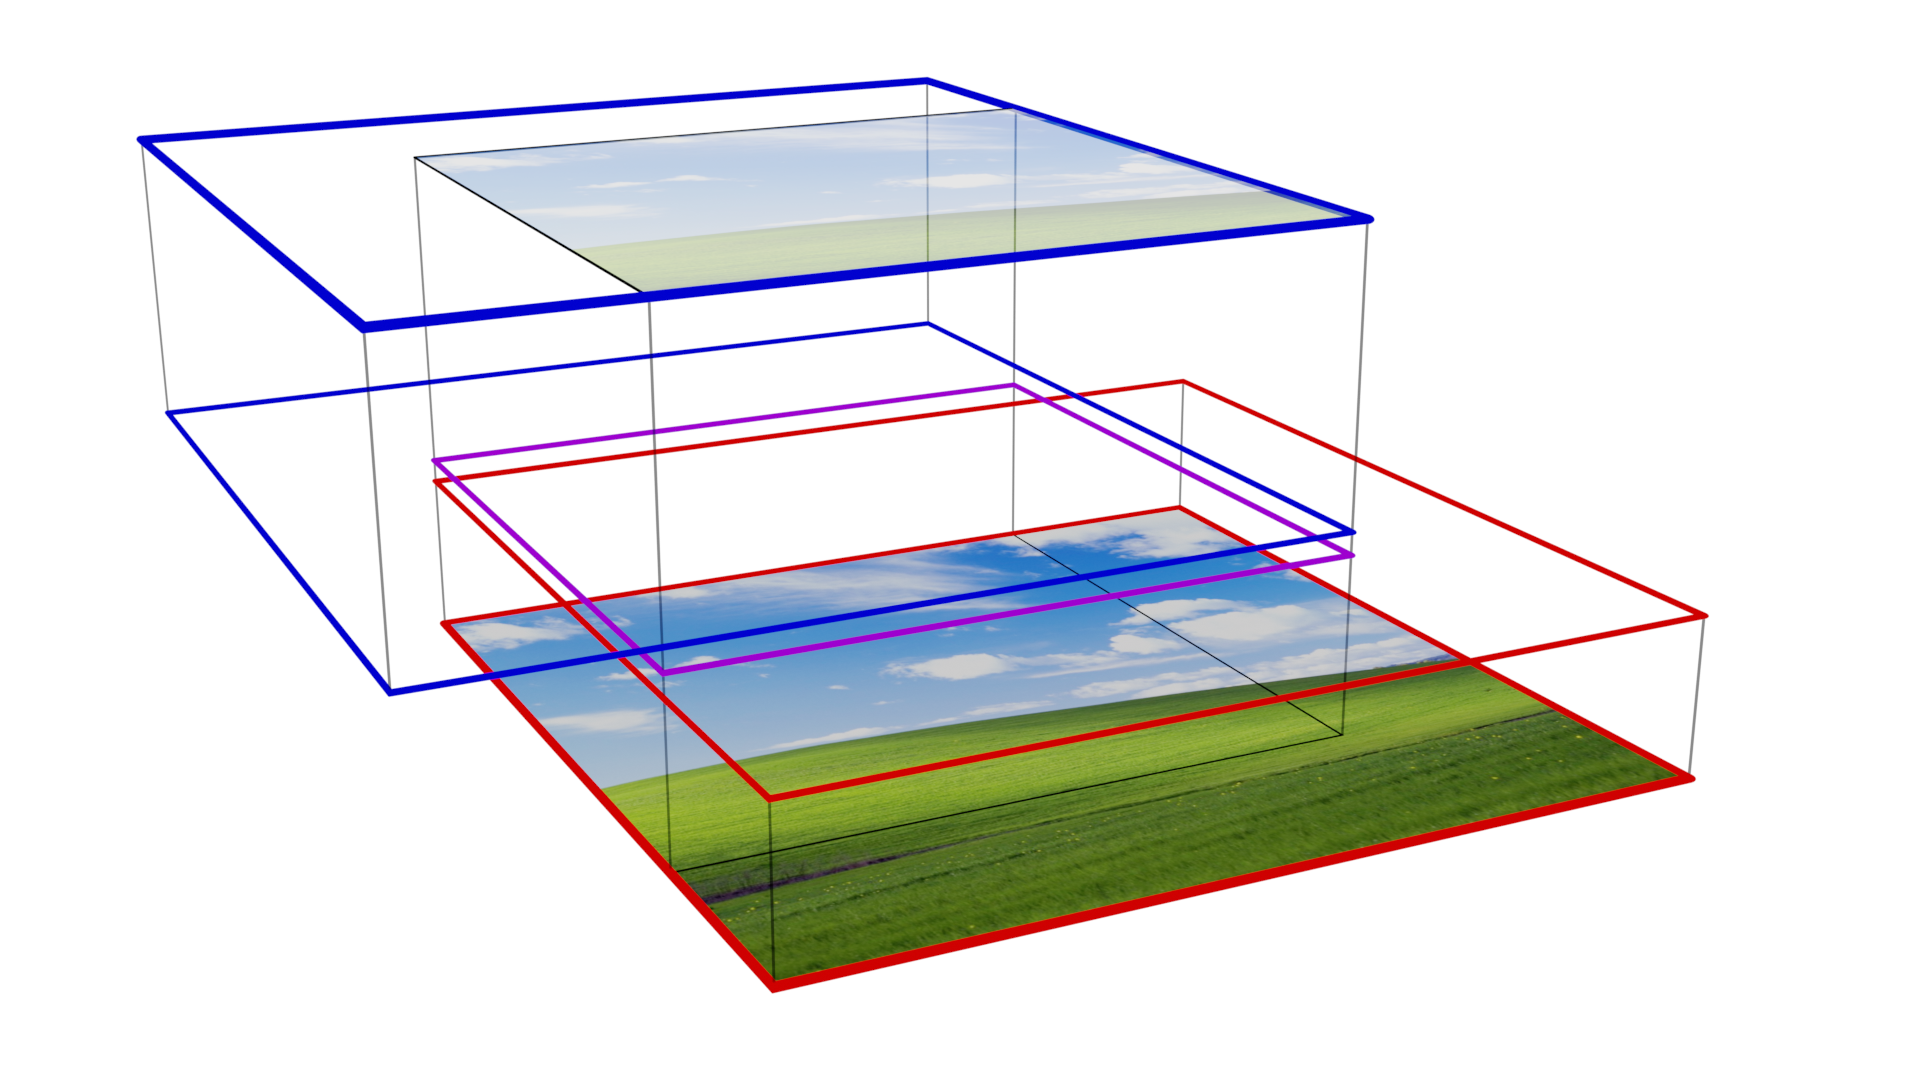
\includegraphics[width=0.9\textwidth]{bbox-compute}
    \end{center}
    \caption{Computing the bounding box for an intermediate layer.  In the first pass, the
    filter/layer above provides a bounding box (rendered in {\color{blue} blue}); in the second, the
    filter/layer below provides another bounding box (rendered in {\color{red} red}).  The region we
    have to compute (rendered in {\color{violet} purple}) is bounded by the union of these
    bounds.}\label{fig:bbox-compute}
\end{figure}

\subsection{Final Notes}

Conceptually, the design employed by this prototype is relatively simple, but \verb|wgpu|'s verbose
API meant that the actual code ended up being surprisingly large and complex (requiring about 1300
source lines of code, most of which is just calling \verb|wgpu|'s API).  This complexity appears to
be unavoidable, so, in a real image editor, I strongly recommend creating a hard abstraction boundary
around the code that truly needs control of the GPU and let the rest of the editor work at a higher
level of abstraction.



\pagebreak

\section{Comparison of Processing Speed}\label{sec:measurements}

\subsection{Methodology}

In this section, we aim to provide a performance comparison between the three ways images can be
processed: CPU, GPU compute passes and GPU render passes (see Section~\ref{sec:compute-types}).  In
order to provide a fair comparison, all tests are running exactly the same implementation algorithm
for adjusting the brightness/contrast of images.  The render pass version is exactly the same as
that used by this project.  Brightness/contrast was chosen because it is reasonably hard to compute:
it isn't trivial to compute (like, say, colour inversion) or very complex to compute (like, say,
Gaussian blur).  It is also indicative of image editing at large: the average modified image
contains lots of simple operations like compositing and colour adjustments, but very few complex
operations such as blurs.

Each device/compute combination was tested on various sizes of images, from 1 mega-pixel to 10
mega-pixels.  All the images have a height of 1000 pixels, and change their width to achieve the
desired size.  GPU compute passes store pixels as a flat array of 32-bit floats, whereas GPU render
passes use 8-bit textures, sampled as floats between 0 and 1.  To keep the comparison fair, the CPU
is measured twice: once storing the images as 32-bit floats (\verb|f32|) and the other as 8-bit
(unsigned) integers (\verb|u8|)---though this turned out to make nearly no difference to the speed.
GPU compute stops at 8 mega-pixels, because any larger images exceed \verb|wgpu|'s maximum buffer
size.  CPU code is compiled for maximum compatibility (as would be done in a proper image editor)
but are fully multi-threaded, taking advantage of as many cores as are available.

Measuring GPU operations is non-trivial, because GPUs are very asynchronous; the CPU-side function
that sends commands to the GPU returns immediately, so in order to get accurate measurements we must
\emph{force} the CPU to block and wait for the GPU to finish executing.

Additionally, we want to only measure the speed of brightness/contrast, without including any other
overhead from interacting with the GPU.  To achieve this, each test is run twice: once for the full
test, and once as a `control' (i.e.\ do everything in the full test \emph{except} the actual
processing).  The control and full tests are both run 100 times for every data-point, with the
values in the graph being the differences of the two averages.  All test cases are run from a single
Rust program, which handles all of these rules.

\subsubsection{Devices Tested}

There are two general types of computer used for image editing; desktops and laptops.  These have
very different performance characteristics: desktop computers prioritise performance over power
efficiency (favouring faster but power hungry processors like dedicated graphics cards), whereas
laptops must be very careful about energy consumption since batteries with large capacity are both
heavy and expensive.

\begin{figure}
    \begin{center}
        \begin{tabular}{ r | c | l }
                & Laptop & Desktop \\
            \hline
            CPU & Intel i7-8550U      & AMD Ryzen 5600X \\
            Cores/Clock & 8 cores, at 4GHz & 12 cores, at 4.6GHz \\
            CPU memory & 8GB & 16GB \\
            \hline
            GPU & Intel UHD Graphics 620 & Nvidia GTX 1060 \\
            GPU memory & 1.5GB (shared with CPU) & 6GB (dedicated) \\
            \hline
            Operating System & Arch Linux & Ubuntu 20.04 \\
            \hline
        \end{tabular}
    \end{center}
    \caption{Comparison of the laptop and desktop computers used for
    testing.}\label{fig:test-computers}
\end{figure}

Figure~\ref{fig:test-computers} gives a comparison of the two computers tested.  Both are
medium-range computers but are optimised for compiling code rather than graphics, so their CPUs are
much more high-end than their corresponding GPUs.  Therefore, if there is any bias in the results,
it will be in favour of the CPU operations.

To reduce measurement interference, both computers were running no other programs while running the
benchmarks (except a terminal emulator and a tiling window manager, which are practically
unavoidable).  Both computers have unmodified performance settings, as would be representative for
a production image editor.

\subsection{Results}

\begin{sidewaysfigure}
    
    \centering
    \begin{minipage}{0.5\textwidth}
        \centering
        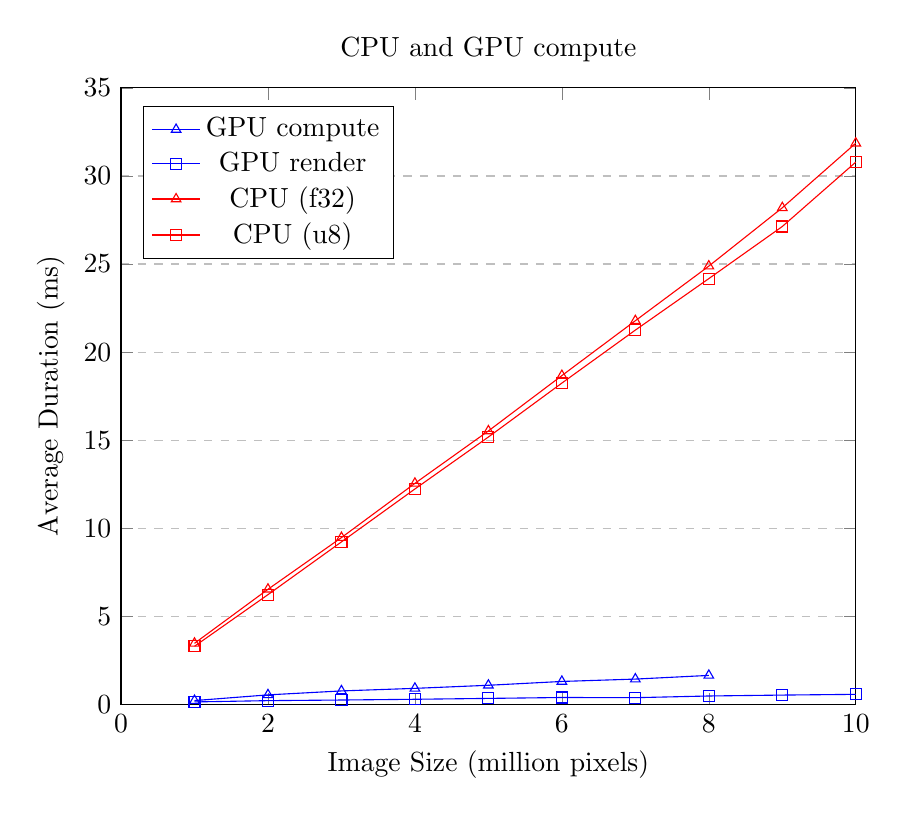
\begin{tikzpicture}
\begin{axis}[
    width=0.9\textwidth,
    title={ CPU and GPU compute },
    xlabel={ Image Size (million pixels) },
    ylabel={ Average Duration (ms) },
    xmin=0, xmax=10,
    ymin=0, ymax=35,
    xtick={ 0, 2, 4, 6, 8, 10 },
    ytick={ 0, 5, 10, 15, 20, 25, 30, 35 },
    legend pos=north west,
    ymajorgrids=true,
    grid style=dashed,
]
\addplot[color=blue, mark=triangle]
    coordinates { (1, 0.22092)(2, 0.54419)(3, 0.76860)(4, 0.91447)(5, 1.08940)(6, 1.30625)(7, 1.44089)(8, 1.64926) };
    \addlegendentry{ GPU compute }
\addplot[color=blue, mark=square]
    coordinates { (1, 0.14417)(2, 0.21686)(3, 0.25206)(4, 0.29447)(5, 0.34409)(6, 0.39529)(7, 0.38552)(8, 0.48120)(9, 0.53287)(10, 0.57458) };
    \addlegendentry{ GPU render }
\addplot[color=red, mark=triangle]
    coordinates { (1, 3.47084)(2, 6.53828)(3, 9.47210)(4, 12.55104)(5, 15.52631)(6, 18.66772)(7, 21.78249)(8, 24.88317)(9, 28.19262)(10, 31.86050) };
    \addlegendentry{ CPU (f32) }
\addplot[color=red, mark=square]
    coordinates { (1, 3.30196)(2, 6.23417)(3, 9.22780)(4, 12.23266)(5, 15.18175)(6, 18.24306)(7, 21.25063)(8, 24.17285)(9, 27.13145)(10, 30.78438) };
    \addlegendentry{ CPU (u8) }

\end{axis}
\end{tikzpicture}
    \end{minipage}\hfill
    \begin{minipage}{0.5\textwidth}
        \centering
        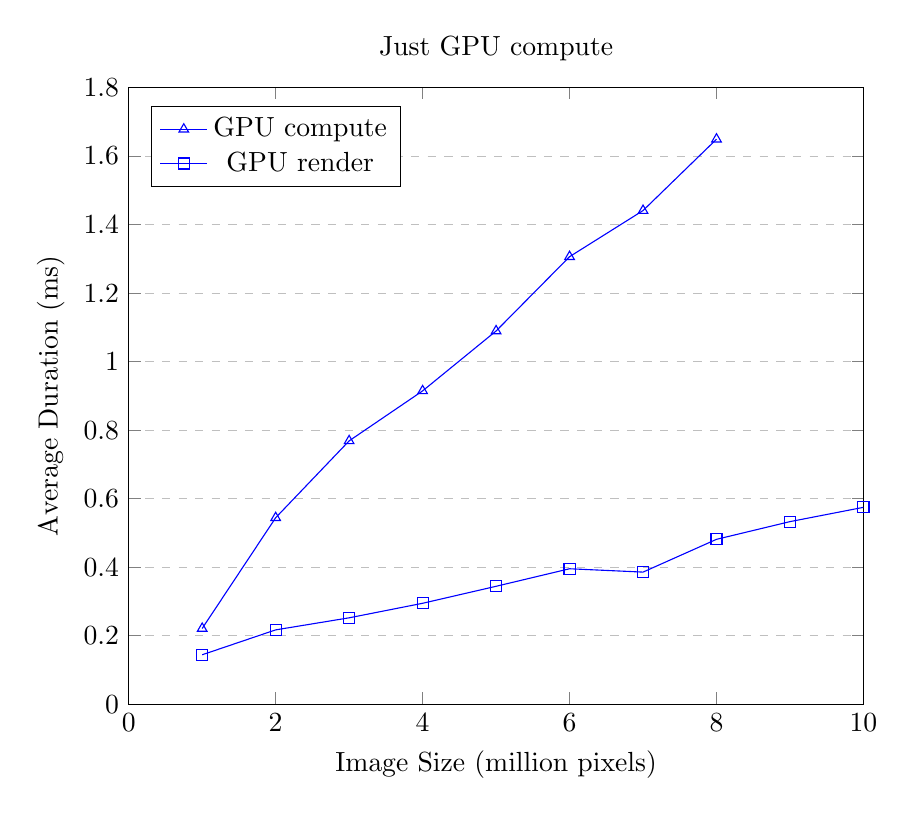
\begin{tikzpicture}
\begin{axis}[
    width=0.9\textwidth,
    title={ Just GPU compute },
    xlabel={ Image Size (million pixels) },
    ylabel={ Average Duration (ms) },
    xmin=0, xmax=10,
    ymin=0, ymax=1.8,
    xtick={ 0, 2, 4, 6, 8, 10 },
    ytick={ 0, 0.2, 0.4, 0.6000000000000001, 0.8, 1, 1.2, 1.4, 1.5999999999999999, 1.7999999999999998 },
    legend pos=north west,
    ymajorgrids=true,
    grid style=dashed,
]
\addplot[color=blue, mark=triangle]
    coordinates { (1, 0.22092)(2, 0.54419)(3, 0.76860)(4, 0.91447)(5, 1.08940)(6, 1.30625)(7, 1.44089)(8, 1.64926) };
    \addlegendentry{ GPU compute }
\addplot[color=blue, mark=square]
    coordinates { (1, 0.14417)(2, 0.21686)(3, 0.25206)(4, 0.29447)(5, 0.34409)(6, 0.39529)(7, 0.38552)(8, 0.48120)(9, 0.53287)(10, 0.57458) };
    \addlegendentry{ GPU render }

\end{axis}
\end{tikzpicture}
    \end{minipage}
    
    \caption{Time required to adjust brightness/contrast on a mid-range desktop computer, containing
    a 12-core 4.6GHz AMD Ryzen 5600X, 16GB of RAM and an Nvidia GTX 1060 (6GB) for the
    GPU.}\label{fig:pc-results}
\end{sidewaysfigure}

\begin{sidewaysfigure}
    
    \centering
    \begin{minipage}{0.5\textwidth}
        \centering
        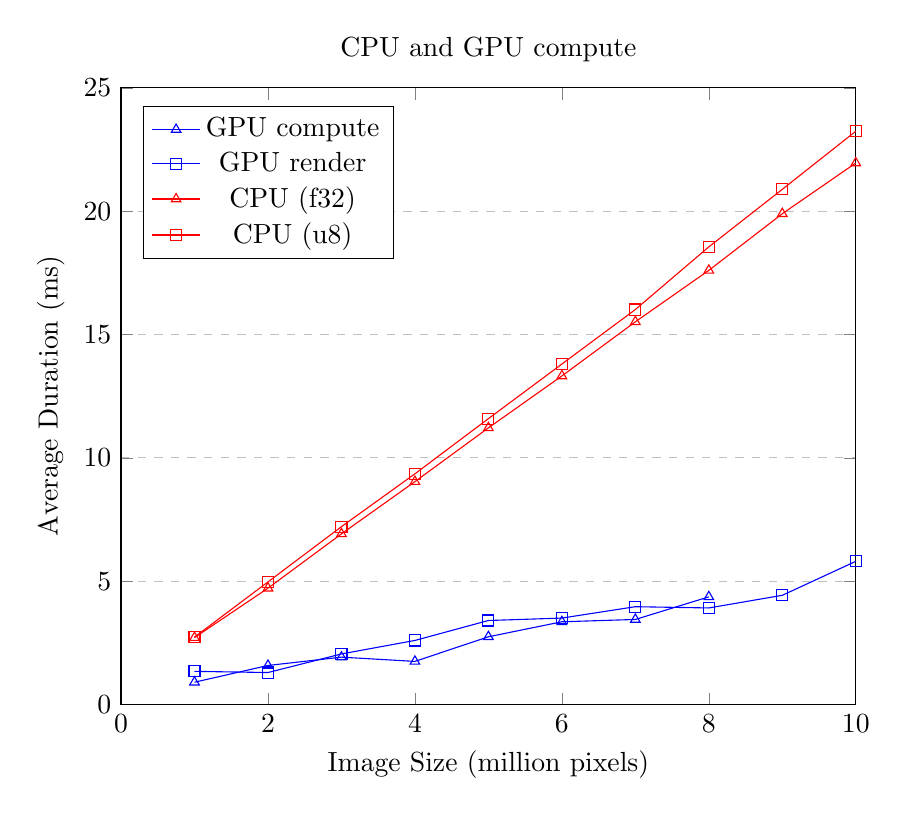
\begin{tikzpicture}
\begin{axis}[
    width=0.9\textwidth,
    title={ CPU and GPU compute },
    xlabel={ Image Size (million pixels) },
    ylabel={ Average Duration (ms) },
    xmin=0, xmax=10,
    ymin=0, ymax=25,
    xtick={ 0, 2, 4, 6, 8, 10 },
    ytick={ 0, 5, 10, 15, 20, 25 },
    legend pos=north west,
    ymajorgrids=true,
    grid style=dashed,
]
\addplot[color=blue, mark=triangle]
    coordinates { (1, 0.90263)(2, 1.58113)(3, 1.91813)(4, 1.74606)(5, 2.74458)(6, 3.35235)(7, 3.44693)(8, 4.36352) };
    \addlegendentry{ GPU compute }
\addplot[color=blue, mark=square]
    coordinates { (1, 1.34261)(2, 1.29489)(3, 2.04895)(4, 2.59564)(5, 3.40430)(6, 3.50268)(7, 3.96413)(8, 3.91326)(9, 4.42554)(10, 5.80358) };
    \addlegendentry{ GPU render }
\addplot[color=red, mark=triangle]
    coordinates { (1, 2.71023)(2, 4.71490)(3, 6.91680)(4, 9.03517)(5, 11.21430)(6, 13.31981)(7, 15.51552)(8, 17.60063)(9, 19.89679)(10, 21.95434) };
    \addlegendentry{ CPU (f32) }
\addplot[color=red, mark=square]
    coordinates { (1, 2.73190)(2, 4.96857)(3, 7.20919)(4, 9.35169)(5, 11.58739)(6, 13.80271)(7, 16.01268)(8, 18.55296)(9, 20.88554)(10, 23.24167) };
    \addlegendentry{ CPU (u8) }

\end{axis}
\end{tikzpicture}
    \end{minipage}\hfill
    \begin{minipage}{0.5\textwidth}
        \centering
        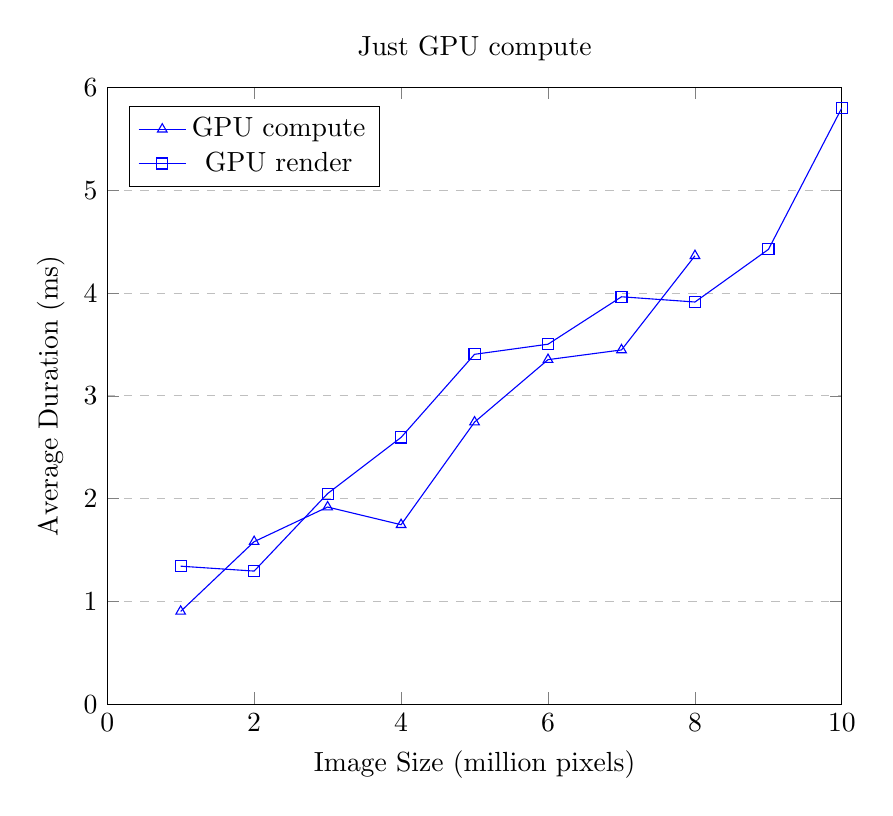
\begin{tikzpicture}
\begin{axis}[
    width=0.9\textwidth,
    title={ Just GPU compute },
    xlabel={ Image Size (million pixels) },
    ylabel={ Average Duration (ms) },
    xmin=0, xmax=10,
    ymin=0, ymax=6,
    xtick={ 0, 2, 4, 6, 8, 10 },
    ytick={ 0, 1, 2, 3, 4, 5, 6 },
    legend pos=north west,
    ymajorgrids=true,
    grid style=dashed,
]
\addplot[color=blue, mark=triangle]
    coordinates { (1, 0.90263)(2, 1.58113)(3, 1.91813)(4, 1.74606)(5, 2.74458)(6, 3.35235)(7, 3.44693)(8, 4.36352) };
    \addlegendentry{ GPU compute }
\addplot[color=blue, mark=square]
    coordinates { (1, 1.34261)(2, 1.29489)(3, 2.04895)(4, 2.59564)(5, 3.40430)(6, 3.50268)(7, 3.96413)(8, 3.91326)(9, 4.42554)(10, 5.80358) };
    \addlegendentry{ GPU render }

\end{axis}
\end{tikzpicture}
    \end{minipage}
    
    \caption{Time required to adjust brightness/contrast on a mid-range laptop computer, containing
    an 8-core 4.0GHz Intel i7-8550U, 8GB of RAM and integrated graphics for the
    GPU.}\label{fig:laptop-results}
\end{sidewaysfigure}

The results are plotted in Figures~\ref{fig:pc-results} and \ref{fig:laptop-results} (for desktop
and laptop, respectively).  All four tests are shown on the left hand graph, while the right hand
graph shows a zoomed version of just the GPU's results.  

\subsubsection{Comparisons}

In both cases, the GPU is substantially faster than the CPU.  For normal image sizes (2-3
mega-pixels), GPU render passes are 3.6x or 28.7x (laptop or desktop, respectively) faster than the
fastest CPU operations.

Considering just GPU operations, render passes are roughly 3x faster than compute on the desktop,
but are the same speed on the laptop.  It would appear that the laptop's GPU is being throttled,
either to reduce heat or to preserve battery life, and this is preventing the GPU from running at
its full capacity.  It is entirely possible to disable throttling on a laptop, but a production
image editor has to use the computer it is given, with whatever configuration it is in.
Additionally, disabling throttling will have a disastrous effect on battery life, which is very
undesirable.

Finally, the desktop's dedicated GPU appears to be roughly 7x faster than the integrated GPU in the
laptop.  This is unsurprising given the difference in design requirements (optimising for raw
performance or power efficiency).

\subsubsection{Interpretation}

An image editor targeting 60 frames per second has at most 16.6ms to perform both the image
processing and the GUI rendering.  Therefore, the vital question is: \emph{how much image processing
can we do within a frame?}  The more processing is possible within a frame, the larger the image a
user can edit before the editor starts having a noticeable delay.

In order to get some concrete numbers, let us assume that 10ms of the 16.6ms frame budget can be
given to image editing.  This seems reasonable; drawing a GUI is likely to be significantly faster
than the image processing, and the GUI layout can be run on the CPU in parallel to the image
processing on the GPU.  Generating the GPU commands takes well under a millisecond, which is largely
negligible compared to the image processing.  We could possibly budget more than 10ms, but having a
buffer of a few milliseconds is useful so that any unexpected delays don't cause frames to be
dropped.

There are two main image sizes of note: images of up to 2 mega-pixels are very common (1920
$\times$ 1080 is `High Definition'), and very few images exceed 8 mega-pixels (the standard `4k'
resolution is 3840 $\times$ 2160).

The dedicated GPU takes roughly 0.2ms and 0.5ms for 2 and 8 mega-pixel images (respectively).
Therefore, on a desktop with dedicated graphics, we can comfortably perform 20 to 50 GPU operations
within a frame.

Laptops are, as expected, much more limited, taking roughly 1.1ms and 4ms for 2 and 8 mega-pixel
images (respectively).  1ms gives around 10 operations per frame, which is likely enough for most
cases.  4ms gives us just over 2 operations per frame, which is very limiting.  If users do edit 4k
images on a mid-range laptop, they should probably expect a maximum 30 frames per second.



\pagebreak

\section{Conclusion}\label{sec:conclusion}

\subsection{This Project}

This project set out to determine the feasibility of using GPU-acceleration to create a
non-destructive image editor, where the update latency is low enough that, upon each update to the
model, a new processed image is ready by the time the next frame gets drawn.  To target 60 frames
per second, an image editor must have a new frame ready every 16.6ms, putting a tight time limit on
the image processing.

Determining the feasibility boils down to answering two questions:

\begin{enumerate}
    \item Is it feasible to design such an editor without huge amounts of complexity?
    \item Are consumer GPUs fast enough to perform this much computation with low enough latency?
\end{enumerate}

To answer (1), a prototype for the `core' of an image editor was designed and implemented, as
described in Section~\ref{sec:implementation}.  This prototype can process images (specified
according to the model of layers and filters) and, whilst the implementation process involved a lot
of fiddly GPU access, the resulting design is conceptually relatively simple.  Additionally, it
seems that much, if not all, of the GPU-related complexity can be encapsulated into one component of
a larger image editor, thus containing the complexity.

To answer (2), we measured the performance of processing the same image filter (brightness/contrast)
using several different processing methods (as described in Section~\ref{sec:compute-types}) and
across different devices, as described in Section~\ref{sec:measurements}.  This also concluded
positively, with discrete GPUs being easily fast enough to hit 60fps reliably, whereas integrated
GPUs in laptops being fast enough that, with some strategic caching of intermediate layers, the
overall editor will still run smoothly.

Personally, I consider this project to be success in its goals.  We do not have the ideal image
editor yet, but this project has shown that it is indeed very likely to be possible.  We also know
that to run well on laptops, it is worthwhile to aggressively optimise the amount of processing
required from the GPU.

\subsection{Next Steps}\label{sec:next-steps}

There are many other parts of building a GPU-accelerated, non-destructive image editor that
haven't been covered by this project.  In a production editor, all of the omissions described in
Section~\ref{sec:omissions} need to be covered, but most of these are implementation details which
simply add complexity to the implementation without needing any design work.  Three obvious areas
that need more design work are undo/redo, masks and brushes.

\subsubsection{Undo/Redo}

GPU-accelerated undo/redo requires us to be able to switch between different versions of the same
layer texture.  The naive approach would be to store a texture containing a full copy of each
version of the changed texture, but this consumes wildly more space than needed.  A proper undo/redo
system needs a way to only store the parts of texture that actually changed, but in such a way that
texture versions can be recovered efficiently.

\subsubsection{Masks}

Masks are not difficult to implement, but they don't immediately incorporate cleanly into the image
model we've given, because they are a filter that takes \emph{two} source layers as input.
Additionally, one of these is a grey-scale layer, which requires all effects to handle different
colour layouts.

\subsubsection{Brushes}

Brushes are a requirement for any image editor, but they are inherently destructive since they
paint over the contents of the layer.  Therefore, a design decision has to be made on how to
incorporate them into the non-destructive model.  In theory, each brush-stroke could create its own
new layer, which would be fully non-destructive but extremely unwieldy in practice.



\pagebreak

\begin{thebibliography}{99}

    \bibitem{khronos} The Khronos Group. \emph{https://www.khronos.org/}
    \bibitem{opengl} Open Graphics Library (OpenGL). \emph{https://www.opengl.org/}
    \bibitem{vulkan} Vulkan API. \emph{https://www.vulkan.org/}
    \bibitem{metal} Metal Graphics API. \emph{https://developer.apple.com/metal/}
    \bibitem{directx} DirectX Graphics API (Wikipedia). \\
        \emph{https://en.wikipedia.org/wiki/DirectX}
    \bibitem{moltenvk} MoltenVK (GitHub). \emph{https://github.com/KhronosGroup/MoltenVK}
    \bibitem{moltengl} MoltenGL (GitHub). \emph{https://moltengl.com/moltengl/}
    \bibitem{opencl} Open Compute Language (OpenCL). \emph{https://www.khronos.org/opencl/}
    \bibitem{webgpu} WebGPU specification. \emph{https://www.w3.org/TR/webgpu/}
    \bibitem{wgpu} \verb|wgpu| repository. \emph{https://github.com/gfx-rs/wgpu}
    \bibitem{photoshop-users} Photoshop's estimated user numbers. \\
        \emph{https://prodesigntools.com/number-of-creative-cloud-subscribers.html}
    \bibitem{adobe-facts} Adobe fast facts. \emph{https://www.adobe.com/about-adobe/fast-facts.html}
    \bibitem{smart-obj} Smart Objects (Photoshop). \\
        \emph{https://helpx.adobe.com/photoshop/using/create-smart-objects.html}
    \bibitem{photoshop-gpu} Vulkan API. \\
        \emph{https://helpx.adobe.com/photoshop/kb/photoshop-cc-gpu-card-faq.html}
    \bibitem{photoshop-wiki} Adobe Photoshop (Wikipedia). \\
        \emph{https://en.wikipedia.org/wiki/Adobe\_Photoshop}
    \bibitem{first-gpu} GeForce 256 (first consumer GPU). \\
        \emph{https://en.wikipedia.org/wiki/GeForce\_256}
    \bibitem{gimp} The GNU Image Manipulation Program. \emph{https://gimp.org}
    \bibitem{gimp-faq} GIMP FAQ. \emph{https://www.gimp.org/docs/userfaq.html}
    \bibitem{gimp-2.10} GIMP 2.10 release notes. \\
        \emph{https://www.gimp.org/news/2018/04/27/gimp-2-10-0-released/}
    \bibitem{darktable} Darktable. \emph{https://www.darktable.org/}
    \bibitem{blender} Blender. \emph{https://www.blender.org/}
    \bibitem{fast-blur} Fast GPU blur algorithms (VentureBeat). \\
        \emph{https://venturebeat.com/2017/07/13/an-investigation-of-fast-real-time-gpu-based-image-blur-algorithms/}
    \bibitem{kawase-blur} Kawase and Dual blur filters. \\
        \emph{https://community.arm.com/cfs-file/\_\_key/communityserver-blogs-components-weblogfiles/00-00-00-20-66/siggraph2015\_2D00\_mmg\_2D00\_marius\_2D00\_notes.pdf}

\end{thebibliography}

\end{document}
